\documentclass[a4paper, 12pt]{article}
\usepackage[utf8]{inputenc}
\usepackage[lmargin=3cm, tmargin=3cm, rmargin=2cm, bmargin=2cm]{geometry}
\usepackage[onehalfspacing]{setspace}
\usepackage[T1]{fontenc}
\usepackage[brazil]{babel}

%%%\usepackage{amssymb, amsmath, mathptmx}%bigominus

\usepackage{wasysym}%male and female

\usepackage{graphicx, graphics, xcolor, comment, enumerate, multirow, multicol, indentfirst}

\usepackage{amsmath, amsthm, amsfonts, amssymb, dsfont, mathtools}
\everymath{\displaystyle} 

\usepackage{blindtext}

\usepackage[round]{natbib}
\bibliographystyle{apalike}

\usepackage{hyperref}

%Code packages:
\usepackage{listings}
\usepackage{xcolor}

%New colors defined below
\definecolor{codegreen}{rgb}{0,0.6,0}
\definecolor{codegray}{rgb}{0.5,0.5,0.5}
\definecolor{codepurple}{rgb}{0.58,0,0.82}
\definecolor{backcolour}{rgb}{0.95,0.95,0.92}

%Code listing style named "mystyle"
\lstdefinestyle{mystyle}{
  backgroundcolor=\color{backcolour},   commentstyle=\color{codegreen},
  keywordstyle=\color{magenta},
  numberstyle=\tiny\color{codegray},
  stringstyle=\color{codepurple},
  basicstyle=\ttfamily\footnotesize,
  breakatwhitespace=false,         
  breaklines=true,                 
  captionpos=b,                    
  keepspaces=true,                 
  numbers=left,                    
  numbersep=5pt,                  
  showspaces=false,                
  showstringspaces=false,
  showtabs=false,                  
  tabsize=2
}

%"mystyle" code listing set
\lstset{style=mystyle}

\title{Projeto 3: Análise Input-Output (Insumo-Produto)}
\author{
  Gabriel Mota Lima\\
  \texttt{11794870}
  \and
  Herberth Luan Vieira Oliveira\\
  \texttt{12559110}
  \and
  Mateus Queiroz de Souza Daniel\\
  \texttt{11294552}
  \and
  Victor Viana de Oliveira Matos\\
  \texttt{11810821}
  \and
  Vinícius da Costa Collaço\\
  \texttt{11811012}
}


\begin{document}

\maketitle

\section{Tarefas}
\subsection{Exercício 1}

\textit{Considere  uma  economia  dividida  em  três  setores  —  manufatura,  agricultura  e  serviços.   Para  cada  unidade  produzida,  a  manufatura  requer 0.10  unidades  de  outras  companhias  do  mesmo  setor,  0.30  unidades  da agricultura e 0.30 unidades de serviços.  Para cada unidade produzida, agricultura usa 0.20 unidades da sua própria produção, 0.60 unidades da manufatura  e  0.10  unidades  de  serviços.   Para  cada  unidade  produzida,o setor de serviços consome 0.10 unidades dele mesmo, 0.60 unidades da manufatura, mas nenhum produto agrícola.}

\subsubsection{(a)}

\textit {Construa a matriz de consumo para esta economia e determine quais demandas intermediárias são criadas se a agricultura planeja produzir 100 unidades}

Para a construção da matriz de consumo foi utilizado phyton com as bibliotecas numpy e pandas. Primeiramente foi construída uma lista com base no texto do item (a), depois passado para um array numpy para uso futuro. 


\begin{lstlisting}[language=Python, caption=Construção da Matriz Consumo 1.a, label=listing_MatrizConsumo1a] 
import numpy as np

consumo1 = [[0.1,0.6,0.6],[0.3,0.2,0],[0.3,0.1,0.1]]
consumo1 = np.array(consumo1)
\end{lstlisting}

tendo o array, utilizou-se a biblioteca pandas, para ter uma melhor visualização da matriz consumo, ficando com a aparência próxima da vista na Tabela \ref{Matriz_Consumo_1a}

\begin{lstlisting}[language=Python, caption=Construção da Matriz Consumo 1.a - Visualização, label=listing_MatrizConsumo1aViz] 
import numpy as np
import pandas as pd

#matriz de consumo para DF, melhor visualizacao
consumo1_df = pd.DataFrame(consumo1)
dic = { 
        0:'manufatura',
        1:'agricultura',
        2:'servicos'
       } #dicionario para mudar o nome das colunas e linhas
consumo1_df.rename(columns = dic, inplace = True)
consumo1_df.rename(index=dic, inplace=True)
consumo1_df


\end{lstlisting}

\begin{table}[]
\begin{tabular}{clll}
\multicolumn{1}{r}{\textbf{}} & \multicolumn{1}{r}{\textbf{manufatura}} & \multicolumn{1}{r}{\textbf{agricultura}} & \multicolumn{1}{r}{\textbf{serviços}} \\
\textbf{manufatura}           & 0.1                                     & 0.6                                      & 0.6                                   \\
\textbf{agricultura}          & 0.3                                     & 0.2                                      & 0.0                                   \\
\textbf{serviços}             & 0.3                                     & 0.1                                      & 0.1    

\end{tabular}
\caption{Matriz Consumo}
\label{Matriz_Consumo_1a}
\end{table}

\textbf{Demandas Intermediárias}\\

Para a evidenciação de todas as demandas intermediárias criadas, será utilizada aqui a abordagem \textit{round-by-round} proposta no livro \citep{livro_miller}. Nesta abordagem considera-se os efeitos somados de todas as demandas intersetoriais geradas. É necessário esta abordagem pois os setores são interdependentes, por exemplo, a produção da agricultura consome recursos do setor de manufatura, estes concursos que são \textbf{input} para o setor de agricultura representam um \textbf{output} para o setor de manufatura, que para gerar esse \textbf{output} precisa consumir \textbf{inputs} dos outros setores. E assim sucessivamente, e teoricamente esse processo segue infinitamente. Cada um desses pares de \textbf{input-output} representam os \textit{rounds}. A demanda intermediária será obtida portanto com uma aproximação deste somatório teoricamente infinito de todos estes \textbf{inputs} gerados. Como será visto, a matriz de Leontief captura todos estes efeitos sucessivos de demandas geradas.

Tendo a matriz de consumo, para saber as quais as demandas intermediárias são criadas no \textit{round 1} para produzir 100 unidades da agricultura, basta multiplicar esse valor (100), pela coluna da agricultura.
Portanto, para uma demanda final 100 unidades da agricultura, são necessárias 60 unidades da manufatura, 20 unidades da agricultura e 10 unidades de serviços nesta primeira etapa. 

No nosso caso, a matriz de consumo e o vetor demanda final são dados por:

$$\mathrm{C}=\begin{bmatrix}
0.1&0.6&0.6\\
0.3&0.2&0\\
0.3&0.1&0.1
\end{bmatrix}\ \ \ \ \ \ \ \ \ \ \ \ \ \ \mathrm{d}=\begin{bmatrix}
0\\
100\\
0
\end{bmatrix}$$

Então, se escrevermos a discussão acima de forma matricial temos que a \textbf{demanda intermediária do round 1} é:

$$\mathrm{Cd}=\begin{bmatrix}
0.1&0.6&0.6\\
0.3&0.2&0\\
0.3&0.1&0.1
\end{bmatrix}\begin{bmatrix}
0\\
100\\
0
\end{bmatrix}=\begin{bmatrix}
60\\
20\\
10
\end{bmatrix}$$

Porém, a demanda intermediária $\mathrm{Cd}$ é o output no \textit{round 2}. Então a \textbf{demanda intermediária do round 2} é dada por:

$$\mathrm{C^2d}=\mathrm{C\cdot Cd}=\begin{bmatrix}
0.1&0.6&0.6\\
0.3&0.2&0\\
0.3&0.1&0.1
\end{bmatrix}\begin{bmatrix}
60\\
20\\
10
\end{bmatrix}=\begin{bmatrix}
24\\
22\\
21
\end{bmatrix}$$

Pelo mesmo raciocínio, a \textbf{demanda intermediária do round 3} é:

$$\mathrm{C^3d}=\mathrm{C\cdot C^2d}=\begin{bmatrix}
0.1&0.6&0.6\\
0.3&0.2&0\\
0.3&0.1&0.1
\end{bmatrix}\begin{bmatrix}
24\\
22\\
21
\end{bmatrix}=\begin{bmatrix}
28.2\\
11.6\\
11.5
\end{bmatrix}$$

Para o caso da \textbf{demanda intermediária do round 4} temos:

$$\mathrm{C^4d}=\mathrm{C\cdot C^3d}=\begin{bmatrix}
0.1&0.6&0.6\\
0.3&0.2&0\\
0.3&0.1&0.1
\end{bmatrix}\begin{bmatrix}
28.2\\
11.6\\
11.5
\end{bmatrix}=\begin{bmatrix}
16.68\\
10.78\\
10.77
\end{bmatrix}$$

Para a \textbf{demanda intermediária do round 5}:

$$\mathrm{C^5d}=\mathrm{C\cdot C^4d}=\begin{bmatrix}
0.1&0.6&0.6\\
0.3&0.2&0\\
0.3&0.1&0.1
\end{bmatrix}\begin{bmatrix}
16.68\\
10.78\\
10.77
\end{bmatrix}=\begin{bmatrix}
14.59\\
7.16\\
7.15
\end{bmatrix}$$\\



Este processo segue infinitamente, e como pode-se ver pelo padrão formado, a demanda intermediária TOTAL é dada pela seguinte soma:

$$\mathrm{Cd}+\mathrm{C^2d}+\mathrm{C^3d}+\mathrm{C^4d}+\mathrm{C^5d}+\ \dots \ =\begin{bmatrix}
60\\
20\\
10
\end{bmatrix}+\begin{bmatrix}
24\\
22\\
21
\end{bmatrix}+\begin{bmatrix}
28.2\\
11.6\\
11.5
\end{bmatrix}+\begin{bmatrix}
16.68\\
10.78\\
10.77
\end{bmatrix}+\begin{bmatrix}
14.59\\
7.16\\
7.15
\end{bmatrix}+\dots $$


Portanto, a demanda intermediária total é dada por uma série de potências da matriz de consumo multiplicada pelo vetor demanda final, isto é:

$$\boxed{\ demanda\ intermediaria=\left(\mathrm{C}+\mathrm{C^2}+\mathrm{C^3}+\mathrm{C^4}+\mathrm{C^5}+\ \dots \right)\mathrm{d}\ \ }$$

Para que esta soma seja convergente a matriz $\mathrm{C}$ deve satisfazer algumas condições. Seus coeficientes não podem ser negativos e a soma dos coeficientes de cada coluna deve ser menor do que 1. Isto é a soma sempre será convergente, desde que a matriz $\mathrm{C}$ seja produtiva, significando que todos os seus setores são lucrativos, como consta no livro \citep{livro_howard}.

Resumindo, a soma acima converge quando os coeficientes da matriz consumo satisfazem as condições \citep{livro_miller}: 

$$c_{ij}\ge 0\ \ \ \ \ and\ \ \ \ \ \sum _{i=1}^n\left(c_{ij}\right)<1\ {,}\ \ para\ todo\ j$$

Abaixo está o código em python para encontrar por aproximação a demanda intermediária, por meio da soma de potências destacada acima:\\

\begin{lstlisting}[language=Python, caption=Demanda intermediária com soma de potências, label=listing_MatrizLeotiefpot]
demanda_final = [[0],[100],[0]]
demanda_final = np.array(demanda_final)

def calcula_demanda_intermediaria(C, d, n):
  N = len (C)  #Tamanho da matriz consumo para criacao da matriz identidade
  I = np.identity(N) #Matriz identidade NxN
  soma_potencias = I - I

  for i in range(1, n):
    soma_potencias += np.linalg.matrix_power(C,i)
  demanda_intermediaria = np.dot(soma_potencias,d)

  return demanda_intermediaria

calcula_demanda_intermediaria(consumo1, demanda_final, 50)

\end{lstlisting}\\

Abaixo está a saída do código acima, para o caso em que a soma de potências vai até a potência $\mathrm{C^{50}}$:

 \begin{center}
    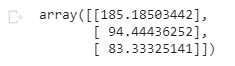
\includegraphics{saida_demanda_intermediaria.PNG}
    
    Figura 2: Saída mostrando a aproximação da demanda intermediária
\end{center}\\

Então, a demanda intermediária é aproximadamente:

$$\boxed{\ \ demanda\ intermediaria\ =\begin{bmatrix}
185.18\\
94.44\\
83.33
\end{bmatrix}\ }$$\\


Portando a demanda intermediária para os produtos do setor de \textbf{manufatura} é de aproximadamente 185.18 unidades, para o setor de \textbf{agricultura} de 94.44 unidades, e de 83.33 unidades para o setor de \textbf{serviços}.

\subsubsection{(b)}

\textit {Obtenha a matriz de Leontief e interprete os seus coeficientes.}\\

\textbf{Leontief com matriz inversa}\\

Para a matriz de Leontief foi inicialmente usada a seguinte definição:

$L = (I - C)^{-1}$

Onde I é a matiz identidade de ordem n, e C é a matriz de consumo $n _\mathrm{x} n$

Então a partir dessa definição foi criada a seguinte função:

\begin{lstlisting}[language=Python, caption=Função Matriz de Leontief, label=listing_MatrizLeotief]

def Leontief (C): #Matriz de Leontief, dado a matriz Consumo n x n
    import numpy as np
    n = len(C)
    I = np.identity(n) #Matriz identidade n x n
    if type(C) == list: C = np.array(C) #Transforma em array se a entrada for lista
    I_C = (I - C)
    L = np.linalg.inv(I_C)#Matriz de Leontief
    return L

\end{lstlisting}

Com a função criada, podemos então obter a matriz de Leontief, chamando a função criada, e como parâmetro de entrada colocamos a matriz criada em \ref{listing_MatrizConsumo1a}

 \begin{center}
    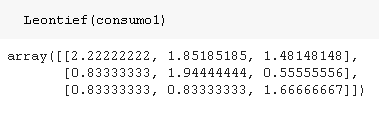
\includegraphics{Leontief1b.PNG}
    
    Figura 1: Saída Da Função Leontief
\end{center}

\textbf{Leontief com Série de Potências}\\

Pelo equilíbrio proposto por Leontief temos:

$$\begin{Bmatrix}
\mathrm{producao}\\
\mathrm{x}
\end{Bmatrix}=\begin{Bmatrix}
\mathrm{demanda}\\
\mathrm{intermediaria}
\end{Bmatrix}+\begin{Bmatrix}
\mathrm{demanda\ final}\\
\mathrm{d}
\end{Bmatrix}$$

Substituindo a expressão da demanda intermediária encontrada no item anterior temos:

$$\mathrm{x}=\left(\mathrm{C}+\mathrm{C^2}+\mathrm{C^3}+\mathrm{C^4}+\mathrm{C^5}+\ \dots \right)\mathrm{d}+\mathrm{d}$$

$$\mathrm{x}=\left(\mathrm{I}+\mathrm{C}+\mathrm{C^2}+\mathrm{C^3}+\mathrm{C^4}+\mathrm{C^5}+\ \dots \right)\mathrm{d}$$

Sendo a expressão que contém a matriz de Leontief da forma $\mathrm{x=Ld}$, então a matriz de Leontief pode ser obtida com a seguinte aproximação de uma série de potências da matriz de consumo:

$$\boxed{\ \mathrm{L}=\mathrm{I}+\mathrm{C}+\mathrm{C^2}+\mathrm{C^3}+\mathrm{C^4}+\mathrm{C^5}+\ \dots \ }$$

Portanto, a matriz de Leontief funciona como um \textbf{multiplicador} da demanda final. Ela leva em conta todas as demandas intermediárias criadas (com o componente $\mathrm{C}+\mathrm{C^2}+\mathrm{C^3}+\mathrm{C^4}+\mathrm{C^5}+\ \dots \ $) e também a demanda final (com o componente $\mathrm{I}$).

Abaixo está o código em python que representa o processo interativo do cálculo da matriz de Leontief usando Série de Potências.\\

\begin{lstlisting}[language=Python, caption=Função Matriz de Leontief por soma de potências, label=listing_MatrizLeotiefpot]
def Leontief_2(C,n):
  import numpy as np
  
  N = len (C) #Tamanho da matriz consumo para criacao da matriz identidade
  I = np.identity(N) #Matriz identidade NxN
  L = I - I #Matriz identidade NxN
  
  for i in range(n):
    L += np.linalg.matrix_power(C,i) #Soma de Potencias n vezes
  return L
\end{lstlisting}\\

Passando a matriz \textit{consumo 1} criada na \textit{Listing 1} para a função \textit{Lentief\_2} acima, tem-se a seguinte saída, para somas que vão até as potências 10, 15, 30 e 50.\\\\\\

Para a soma que vai até $\mathrm{C^{10}}$:

 \begin{center}
    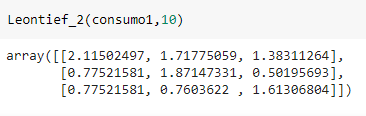
\includegraphics{pot_10.PNG}
    
    Figura 2: Soma até $\mathrm{C^{10}}$
\end{center}\\

Para a soma que vai até $\mathrm{C^{15}}$:

 \begin{center}
    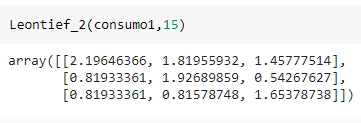
\includegraphics{pot_15.PNG}
    
    Figura 2: Soma até $\mathrm{C^{15}}$
\end{center}\\

Para a soma que vai até $\mathrm{C^{30}}$:

 \begin{center}
    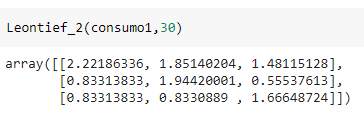
\includegraphics{pot_30.PNG}
    
    Figura 2: Soma até $\mathrm{C^{30}}$
\end{center}\\

Para a soma que vai até $\mathrm{C^{50}}$:

 \begin{center}
    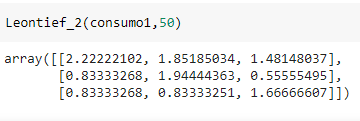
\includegraphics{pot_50.PNG}
    
    Figura 2: Soma até $\mathrm{C^{50}}$
\end{center}

Pode-se notar que a medida que se aumenta a quantidade de potências contidas na soma da série, mais o resultado obtido \textbf{converge} para a matriz de Leontief obtida invertendo-se a matriz $(\mathrm{I-C})$.


\subsubsection{Interpretação dos coeficientes}

Como foi visto, a matriz de Leontief como um todo pode ser interpretada como um multiplicador da demanda final, para se encontrar qual a produção total. Vimos também que a matriz de Leontief tem um componente que leva em conta a demanda final (componente $\mathrm{I}$) e um componente que leva em consideração as demandas intermediárias geradas ($\mathrm{C}+\mathrm{C^2}+\mathrm{C^3}+\mathrm{C^4}+\mathrm{C^5}+\ \dots \ $). Dadas todas estas somas, temos que os elementos da \textbf{diagonal principal} da matriz de Leontief será sempre maior ou igual a 1, pois o setor terá que produzir para atender a sua própria demanda final somado com as demandas intermediárias criadas. Enquanto os outros coeficientes podem assumir qualquer valor maior ou igual a zero, pois são multiplicadores que representam as demandas intermediárias criadas.

Por exemplo, na seguinte matriz:

$$\mathrm{L} = \begin{bmatrix}
l_{11}&l_{12}&l_{13}\\
l_{21}&l_{22}&l_{23}\\
l_{31}&l_{32}&l_{33}
\end{bmatrix} = \begin{bmatrix}
2.22&1.85&1.48\\
0.83&1.94&0.55\\
0.83&0.83&1.66
\end{bmatrix}$$

Considerando a primeira linha, o coeficiente $l_{11}$ é um multiplicador da demanda final pelos produtos do setor 1 e representa o impacto que a demanda final do setor 1 representa na produção do próprio setor 1, $l_{11}$ deve ser maior ou igual a 1 pois o setor 1 deve produzir para atender a sua própria demanda final, somado com a produção para atender as demandas intermediárias. Seguindo o mesmo raciocínio, o coeficiente $l_{12}$ representa por quanto a demanda final pelos produtos do setor 2 é multiplicada para se chegar à quantidade a mais de demanda intermediária pelos produtos do setor 1, isto é, representa o impacto da demanda final pelos produtos do setor 2 na produção do setor 1.

Deste modo, pode-se ver que a magnitude do coeficiente $l_{ij}$ representa o quando a demanda final pelos produtos do setor $j$ afeta a produção do setor $i$. Quanto maior o valor de $l_{ij}$, maior é este impacto, que acontece por meio das demandas intermediárias entre os setores.


\subsubsection{(c)}
\textit {Determine os níveis de produção necessários para satisfazer uma demanda final de 18 unidades para a agricultura, e nenhuma demanda final para os outros setores. Que relação você observa entre a resposta e a matriz de Leontief?}

Para obtenção dos níveis de produção necessários para dada uma certa demanda final, precisamos resolver o seguinte sistemas de equações 

$(I - C)*X = D$ , onde I é a matriz identidade na mesma dimensão da matriz consumo, C é a matriz consumo, X é a matriz com os resultados, e D a matriz coluna com a demanda final. Para resolver esse sistema foi criado a seguinte função:


\begin{lstlisting}[language=Python, caption=Função Calculo da Produção, label=listing_Producao]

def Producao(C,d): #Calculo da producao dado a matriz consumo e demanda
  import numpy as np
  if type(C) == list: C = np.array(C) #Transforma em array se a entrada for lista
  if type(d) == list: d = np.atleast_2d(d).T #Transforma d em matriz coluna se for lista
 
  L = Leontief(C)
  
  #Resolucao de sistema linear via Matriz Leontief
  #Encontrar o x, multiplicacao de matriz (L*d)
  X = np.dot(L,d)

  return X
  
 \end{lstlisting}

para isolar o X, podemos utilizar o inverso da função $(I - C)$, que é exatamente a matriz de Leontief, então como já havíamos criado a função do cálculo de Leontief, a resolução do sistema vai se dar através da multiplicação da matriz de Leontief com a matriz coluna da demanda final

Tendo a função, a matriz de consumo e a lista de entrada referente a uma demanda final de 18 unidades para a agricultura podemos calcular a demanda intermediária, dada por:

\begin{lstlisting}[language=Python, caption=Cálculo da Demanda Intermediária, label=listing_Calc_int]

d_ex1 = [0,18,0]
Producao(consumo1,d_ex1)
  
 \end{lstlisting}

com o código em \ref{listing_Calc_int} temos a seguinte saída

\begin{center}
    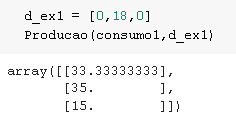
\includegraphics{saida1c.PNG}
    
    Figura 2: Demandas Intermediárias
    
\end{center}

Portanto precisaria de 33.3333 unidades da manufatura, 35 unidade da agricultura e 15 unidades de serviços para uma demanda final de 18 unidades para a agricultura.

Podemos observar uma relação direta entre a demanda intermediária e a matriz de Leontief, se por exemplo multiplicarmos cada elemento da matriz de Leontief calculada anteriormente por 18, temos o seguinte resultado

\begin{center}
    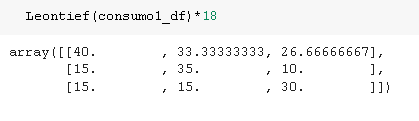
\includegraphics{saida1c_2.PNG}
    
    Figura 3: Leontief * 18
    
\end{center}

a segunda coluna apresenta exatamente o resultado obtido anteriormente, verificando essa relação direta entre a demanda final, a matriz de Leontief e as demandas intermediárias.

\subsection{Exercício 2}

\textit{A matriz de consumo abaixo em dados de insumo-produto da economia norte-americana em 1958, com dados para 81 setores agrupados em 7 grandes setores: (1) produtos domésticos e pessoais não metálicos, (2) produtos metálicos finais (como veículos motorizados), (3) produtos metálicos básicos e mineração, (4) produtos não metálicos básicos e agricultura, (5)energia, (6) serviços e (7) produtos diversos}

$$\begin{bmatrix}
0.1588 & 0.0064 & 0.0025 & 0.0304 & 0.0014 & 0.0083 & 0.1594 \\
0.0057 & 0.2645 & 0.0436 & 0.0099 & 0.0083 & 0.0201 & 0.3413 \\
0.0264 & 0.1506 & 0.3557 & 0.0139 & 0.0142 & 0.0070 & 0.0236 \\
0.3299 & 0.0565 & 0.0495 & 0.3636 & 0.0204 & 0.0483 & 0.0649 \\
0.0089 & 0.0081 & 0.0333 & 0.0295 & 0.3412 & 0.0237 & 0.0020 \\
0.1190 & 0.0901 & 0.0996 & 0.1260 & 0.1722 & 0.2368 & 0.3369 \\
0.0063 & 0.0126 & 0.0196 & 0.0098 & 0.0064 & 0.0132 & 0.0012
\end{bmatrix}$$

inicialmente a matriz de consumo foi transformada em array com as informações do pdf, como não foi possível copiar a matriz direto do pdf, foi necessário um tratamento inicial, e então colocada as informações dessa matriz de consumo na variável (matirz\_ex2), com o seguinte código:

\begin{lstlisting}[language=Python, caption=Criação matriz\_ex2, label=listing_matriz_ex2]

#matriz copiada do pdf
matriz = '.1588.0064.0025.0304.0014.0083.1594.0057.2645.0436
          .0099.0083.0201.3413.0264.1506.3557.0139.0142.0070
          .0236.3299.0565.0495.3636.0204.0483.0649.0089.0081
          .0333.0295.3412.0237.0020.1190.0901.0996.1260.1722
          .2368.3369.0063.0126.0196.0098.0064.0132.0012'
ex2 = []
for i in range(1,50):
  ex2.append(int(matriz.split('.')[i])/10000)
matriz_ex2 = np.array([ex2[:7],ex2[7:14],ex2[14:21],ex2[21:28],ex2[28:35],ex2[35:42],ex2[42:]])

 \end{lstlisting}
 
 tendo o array, podemos utilizar as funções criadas anteriormente para resolver as seguintes questões:
 
 \subsubsection{(a)}
 \textit{Calcule os níveis de produção para satisfazer a demanda final}
 
 $\begin{matrix}
 d = [7400 & 56000 & 10500 &   25000 &   17500 &    196000 &   5000]^T
 \end{matrix}$
 
 Utilizando a Função 'Producao', chegamos a seguinte saída
 
 \begin{center}
    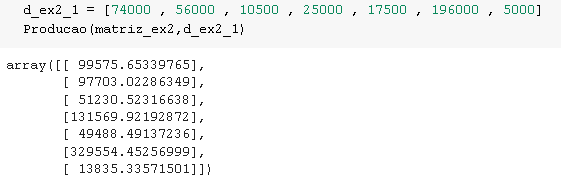
\includegraphics{saida2a.PNG}
    
    Figura 4: Saída Exercício 2 a)
    
\end{center}
 
 Assim temos os níveis de produção intermediária para o ano de 1958
 
 \subsubsection{(b)}
 \textit{Calcule os níveis de produção da seguinte demanda e compare com o resultado anterior.}
  $\begin{matrix}
 d = [99640 & 75548 &  14444 &  33501 & 23527 & 263985 & 6526]^T
 \end{matrix}$
 
 \begin{center}
    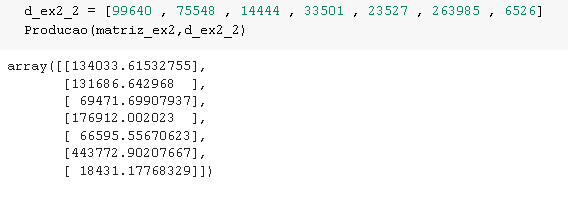
\includegraphics{saida2b.PNG}
    
    Figura 5: Saída Exercício 2 b)
    
\end{center}

Com o mesmo método foi possível calcular os níveis de produção do ano de 1964. Como foi utilizada a mesma matriz de consumo, assim temos a mesma matriz de Leontief nos dois casos. Como os níveis de produção é proporcional à demanda final, dado a mesma matriz de Leontief, observamos que no segundo caso, como temos valores de demanda final maiores, acaba resultando em níveis de produção maiores também.

Isso faz sentido dado o caso onde não temos mudança das demandas intersetoriais. É possível termos mudanças na matriz de consumo, conforme a tecnologia e meios de produção vão mudando, assim certo setor usaria uma quantia diferente intersetorial ao passar do tempo, porém essas mudanças não tendem a ser tão bruta, pois estamos observando o cenário mais macro, então o resultado apresentado faz sentido em termos reais.

\subsection{Exercício 3}

\textit{Na
\href{https://www.ibge.gov.br/estatisticas/economicas/contas-nacionais/9085-matriz-de-insumo-produto.html}{página do IBGE}
há informações sobre o resultado de atividades econômicas.  Leia a explicação.  Depois,clique o link ”Downloads” à esquerda na página, acesse as informações do ano de 2015 e baixe a planilha relativa a 12 setores da economia. Nesta planilha, localize a aba que contém a matriz de consumo e calcule a matriz de Leontief.  Compare o seu resultado com a matriz de Leontief que está na planilha.  Interprete alguns coeficientes da matriz de Leontief.}

No site do IBGE temos as planilhas em formato xls, para tratamento dos dados, e posterior a utilização nas funções previamente criadas, utilizaremos a biblioteca 'pandas' e também a biblioteca 're', a primeira para transformar os dados da planilha excel em um array e a segunda para utilização de expressão regular para tratar o nome das linhas e colunas, essa última para fins estéticos.

\begin{lstlisting}[language=Python, caption=Tratamento Excel, label=listing_trat_excel]

def Tratamento_excel(nome_arquivo,nome_aba): 
  #Funcao para tratar o arquivo excel e devolver um DataFrame limpo para ser utilizado
  
  import pandas as pd
  import re
 
  #Tratamento inicial
  df = pd.read_excel(nome_arquivo,sheet_name=nome_aba,header=3).drop(['Unnamed: 0','Unnamed: 1'],axis=1)
  df = df.dropna()
  df = df.reset_index().drop('index',axis=1)

  #tratar o nome das colunas com Regex
  colunas = []#nome das colunas limpo
  for item in  df.columns: #tira o numero e o '\n' 
    colunas.append(re.sub('(.*\\n)','',item))

  #Renomear colunas e index
  dic_col = dict(zip(df.columns,colunas)) #dicionario para renomear as colunas
  df.rename(columns = dic_col, inplace = True)
  lendf = len(df)
  dic_index = dict(zip(range(0,lendf),colunas))#dicionario para renomear os index
  df.rename(index=dic_index, inplace=True)
  
  return df
  
\end{lstlisting}
  
Assim temos a matriz de consumo com 12 setores do ano de 2015

 \begin{center}
    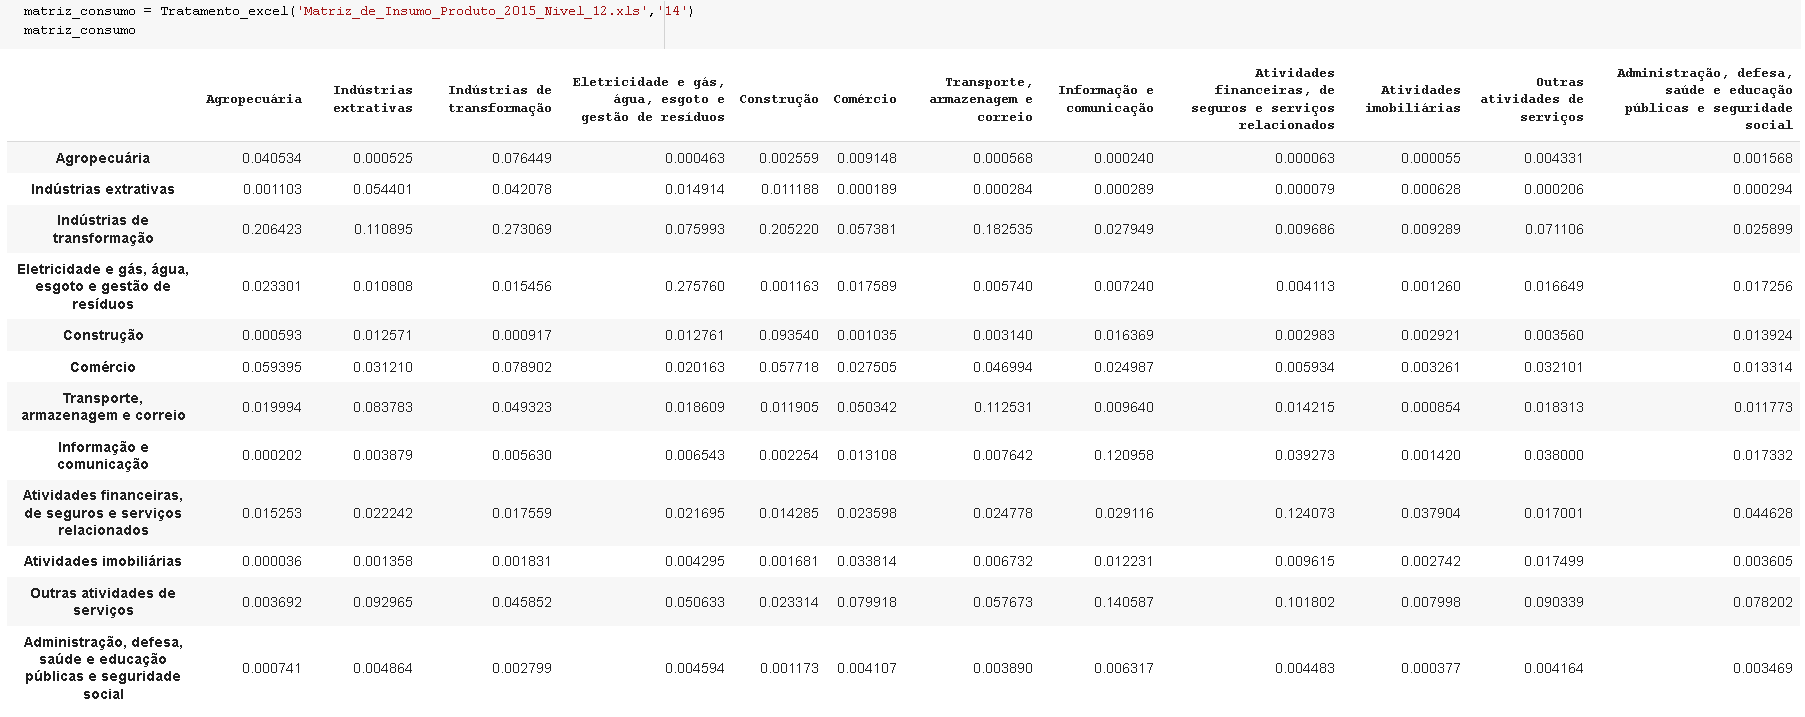
\includegraphics[width=16cm]{consumo_12_2015.PNG}
    
    Figura 6: Matriz de consumo 12 setores de 2015 tratada)
    
\end{center}

Na planilha fornecida do site do IBGE, a aba de número 14, representa a matriz de consumo e a aba de número 15 a matriz de Leontief.

Com a entrada tratada, podemos utilizar a mesma função 'Leontief' para gerarmos a matriz de Leontief dada como entrada a matriz de consumo com 12 setores de 2015.

 \begin{center}
    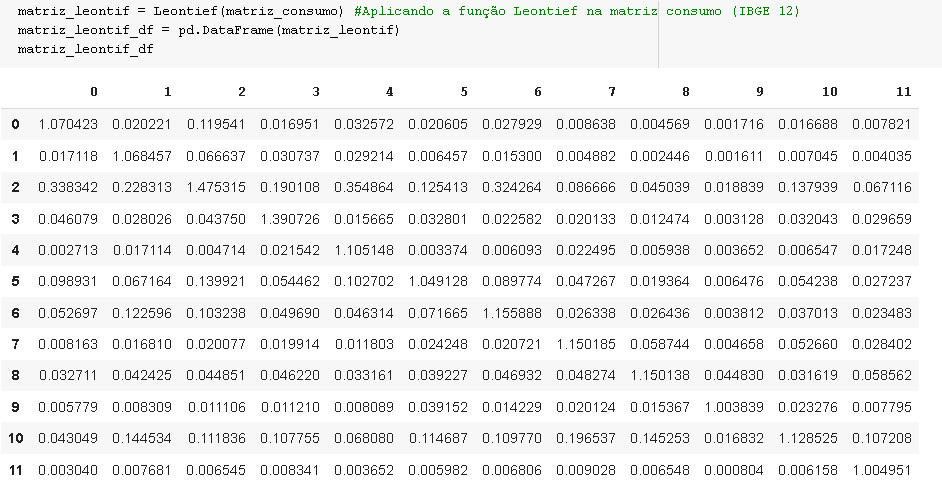
\includegraphics[width=16cm]{Leontief_12_2015.PNG}
    
    Figura 7: Matriz de Leontief 12 setores de 2015 obtidada com a Função Leontief
    
\end{center}

Como temos na planilha fornecida no IBGE a matriz de Leontief na aba 15, podemos comparar a saída anterior com a matriz da aba 15 e verificar o funcionamento da nossa função para o caso real. Porém antes foi criada uma função para extrair a matriz de Leontief direto do excel fornecido do IBGE.

\begin{lstlisting}[language=Python, caption=Leontief direto do excel, label=listing_leontief_excel]
def Leontief_excel(nome_arquivo,nome_aba):

  matriz_consumo = Tratamento_excel(nome_arquivo,nome_aba)
  matriz_leontif = Leontief(matriz_consumo) #Aplicando a funcao Leontief na matriz consumo (IBGE)
  matriz_leontif_df = pd.DataFrame(matriz_leontif)

  #Renomear colunas e index  
  lendf = len(matriz_consumo)
  dic_index = dict(zip(range(0,lendf),matriz_consumo.columns))#dicionario para renomear os index e colunas
  matriz_leontif_df.rename(index=dic_index, inplace=True)
  matriz_leontif_df.rename(columns = dic_index, inplace = True)


  return matriz_leontif_df
\end{lstlisting}

então podemos assim comparar a saída da nossa função com a matriz de Leontief do site do IBGE em poucas linhas:

\begin{center}
    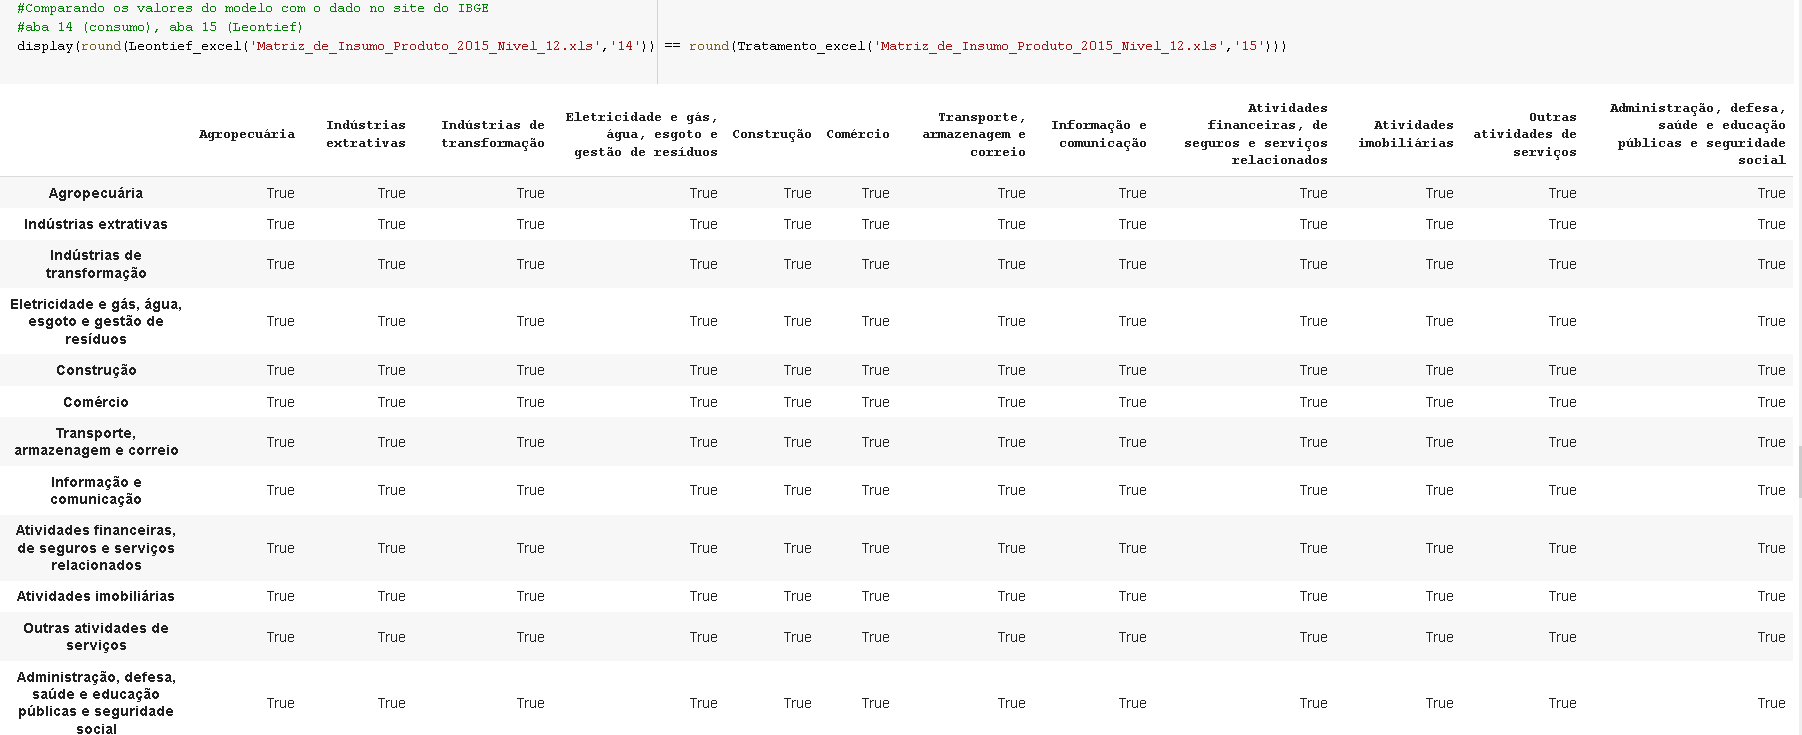
\includegraphics[width=16cm]{Comparacao_Leontief12.PNG}
    
    Figura 8: Comparação da Saída com os dados do IBGE
    
\end{center}

foi necessário arredondar os valores, mas o resultado obtido através das funções construídas condizem com o encontrado na aba 15, do arquivo excel. Comparando valor a valor, todas as comparações deram True, indicando que as duas matrizes, tanto a calculada quanto a fornecida, são iguais.

\subsubsection{Interpretando alguns coeficientes}

Com a matriz de Leontief calculada podemos pegar por exemplo a diagonal principal, (3,3), onde o índice 3 representa o setor de Eletricidade e gás, água, esgoto e gestão de resíduos. Essa diagonal do setor é uma que tem um dos maiores valores, que faz sentido, já que os outros setores precisam dos produtos gerados por esse setor.
Em contra partida a diagonal com o menor valor é a do setor com índice 9, que é o setor de Atividades imobiliárias, que é um setor que não gera tanto impacto nos outros setores, por ser tipo de atividade que não necessariamente empreende tantos produtos diversos, sendo isso normalmente para setores de construção civil.
O ponto a se destacar é que o Brasil é conhecido como um país que trabalha com produtos agropecuários (coluna índice 0) e de acordo com a matriz de Leontief mostra que mesmo sendo o setor econômico principal brasileiro ele não faz gerar aumento de demandas relevantes aos demais setores econômicos quando comparados com setor de indústrias de transformação (coluna índice 2), o que pode-se inferir que a indústria tem forte impacto intersetorial na economia e um relação mais intensa com os demais setores do que o agropecuário.


\section{Estendendo o algorítimo para a planilha de 20 setores e 67 setores}

Conforme foram criados os algorítimos para cálculo da Matriz de Leontief direto da planilha fornecida pelo site do IBGE, podemos fazer o cálculo com o mesmo algoritmo mas para as duas planilhas maiores, tanto a de 20 setores como a de 67 setores.

 \begin{center}
    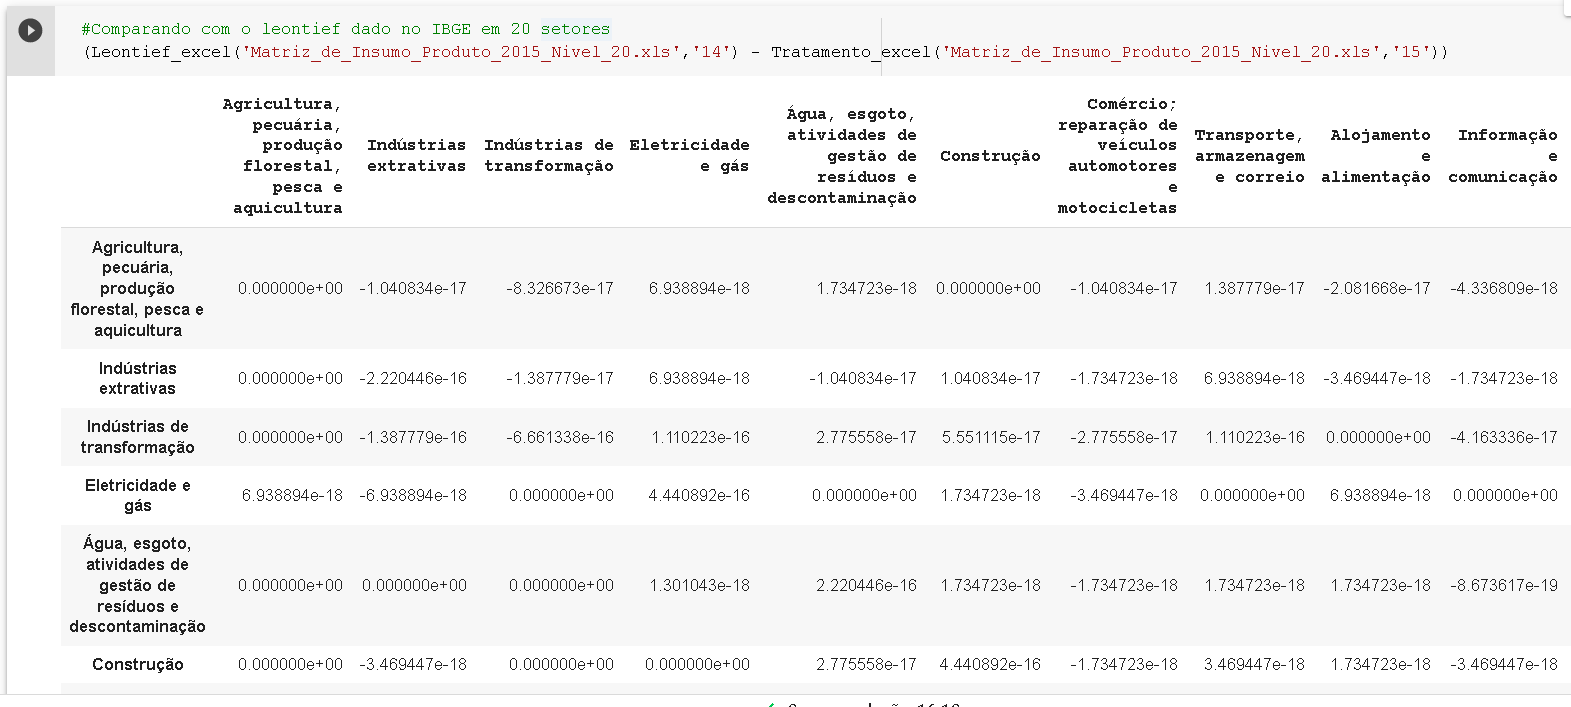
\includegraphics[width=16cm]{saidaExtraA.PNG}
    
    Figura 9: Parte das Matrizes de Leontief Importada e Calculada, diferença entre valores.
    
\end{center}

Como a planilha de 20 setores é muito grande, foi colocada na imagem somente parte da saída, nesse exemplo foi subtraído os elementos correspondentes da Matriz de Leontief Calculada pelo modelo criado, com o input da Matriz de consumo (Aba 14 do arquivo de excel), com a matriz de Leontief fornecida (Aba 15 do arquivo de excel).
Não foi usado o método round, para mostrar a diferença irrisória das duas matrizes

 \begin{center}
    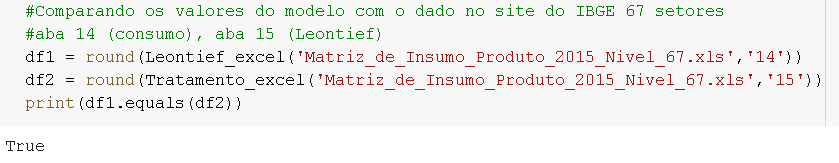
\includegraphics[width=16cm]{saidaExtraB.PNG}
    
    Figura 10: Comparação das Matrizes de Leontief Importada e Calculada, 67 setores.
    
\end{center}

O mesmo foi verificado com a matriz de 67 setores, mostrando que o algoritmo criado para importar e tratar os dados direto da planilha do site do IBGE e também o algoritmo de cálculo da matriz de Leontief, funcionam para qualquer que seja o tamanho, baseado em diferentes setores.

\section{Código Fonte}
\href{https://colab.research.google.com/drive/1Egm5Q4_bd0hEZh8YK9W7ZAZBJh5ALt2e?usp=sharing}{https://colab.research.google.com/drive/1Egm5Q4\_bd0hEZh8YK9W7ZAZBJh5ALt2e}

Código criado em Python, com o Jupyter Notebook em Colab, com as saídas completas
  
\bibliography{ref.bib}

\end{document}
